\label{sec:results}

\subsection{Revisiting Frozen Lake \& Tiger Door}
\label{sec:results:gridworld} 
We evaluate A2D on the gridworlds introduced in Section \ref{sec:prelim}.  Results are shown in Figures \ref{fig:gridworld_asym} and \ref{fig:grid:a2dplot}.  Figure \ref{fig:gridworld_asym} shows that A2D converges to the optimal POMDP reward quickly, and, in a comparable number of interactions to the best-possible convergence of RL in the MDP when using similar hyperparameters to those used for A2D (\emph{RL (MDP)}).  Convergence rates are also similar for high-dimensional images (\emph{A2D (Image)}) and low-dimensional representations (\emph{A2D (Compact)}).  Other methods fail for one, or both, gridworlds.  A2D can also operate with hyperparameters broadly similar to those tuned specifically for RL in the MDP, where tuning is easy.  However, A2D did then benefit from increased batch size, entropy regularization, and reduced $\lambda$ (see Appendix \ref{supp:exp}).  The IL hyperparameters are largely independent of the RL hyperparameters, further simplifying tuning overall.  

\begin{figure*}[!htb]
    \centering
    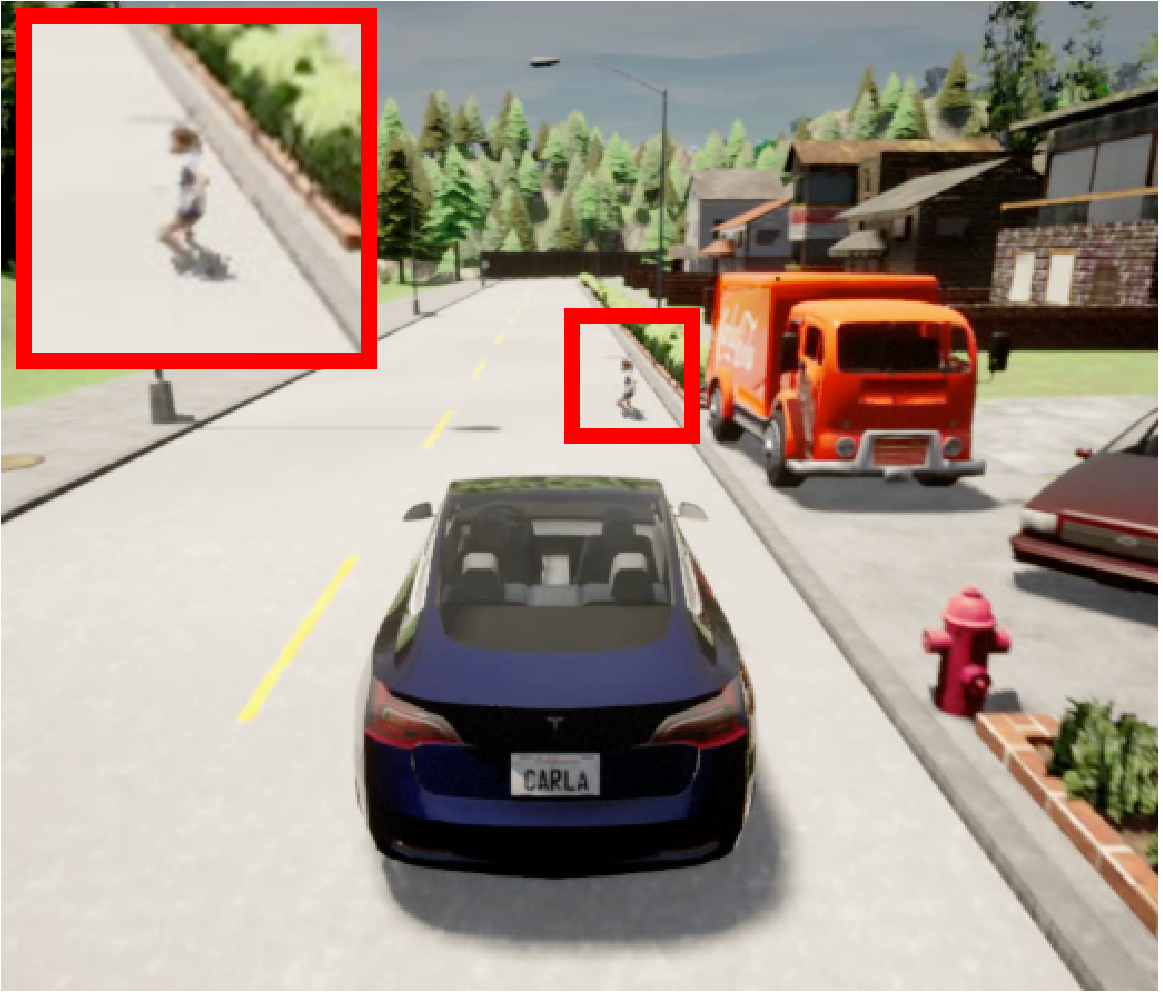
\includegraphics[width=0.245\textwidth]{figures/carla/child_zoom.pdf} \hfill
    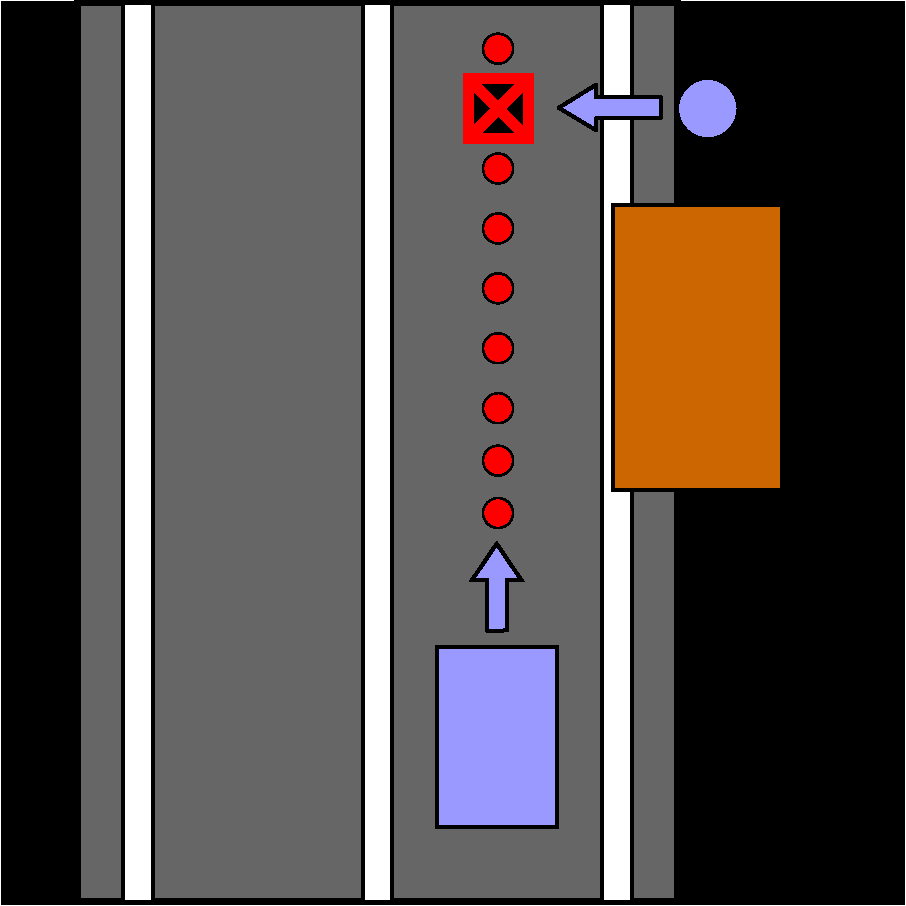
\includegraphics[width=0.2105\textwidth]{figures/carla/compact_state_new_new.pdf} \hfill
    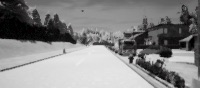
\includegraphics[width=0.48\textwidth]{figures/carla/1_front_view.jpg}
    \caption{Visualizations of the AV scenario.  Left: third-person view showing the egovehicle and child running out.  Center: top-down schematic of the environment and asymmetric information.  Right: front-view camera input provided to the agent.}
    \vspace*{-0.2cm}
    \label{supp:fig:carla:a2dplot:inputs}
\end{figure*}


Figure \ref{fig:grid:a2dplot} shows the divergence between the expert and trainee policies during learning.  \emph{AIL} saturates to a high divergence, indicating that the trainee is unable to replicate the expert.  The divergence in A2D increases initially, as the expert learns using the full-state information.  This rise is due to the non-zero value of $\beta$, imperfect function approximation, slight bias in the gradient estimator, and the tendency of the expert to initially move towards a higher reward policy not representable under the agent.  As the learning develops, and $\beta \tends 0$, the expert is forced to optimize the reward of the trainee.  This, in turn, drives the divergence towards zero, producing a policy that can be represented by the agent.  A2D has therefore created an identifiable expert and implicit policy pair (Definition \ref{def:consistency_pol}), where the implicit policy is also optimal under partial information.  


\subsection{Safe Autonomous Vehicle Learning}
\label{sec:results:carla}
Autonomous vehicle (AV) simulators~\citep{Dosovitskiy17, wymann_torcs_2014, kato_open_2015} allow safe virtual exploration of driving scenarios that would be unsafe to explore in real life.  The inherent complexity of training AV controllers makes exploiting efficient AIL an attractive opportunity~\citep{Chen2019}.  The expert can be provided with the exact state of other actors, such as other vehicles, occluded hazards and traffic lights.  The trainee is then provided with sensor measurements available in the real world, such as camera feeds, lidar and the egovehicle telemetry.  

%CARLA challenge traffic scenario 3 \& 4
The safety-critical aspects of asymmetry are highlighted in context of AVs. Consider a scenario where a child may dart into the road from behind a parked truck, illustrated in Figure \ref{supp:fig:carla:a2dplot:inputs}.  The expert, aware of the position and velocity of the child from asymmetric information, will only brake if there is a child, and will otherwise proceed at high speed.  However, the trainee is unable to distinguish between these scenarios, before the child emerges from, just the front-facing camera.  As the expected expert behavior is to accelerate, the implicit policy also accelerates.  The trainee only starts to brake once the child is visible, by which time it is too late to guarantee the child is not struck.  The expert should therefore proceed at a lower speed so it can slow down or evade the child once visible. This cannot be achieved by naive application of AIL.  

\begin{figure*}[!htb]
    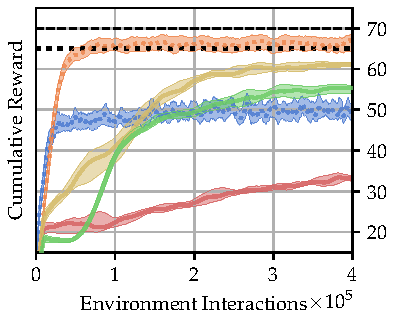
\includegraphics[width=0.315\textwidth]{figures/carla/scenario_1_time_steps_reward_results.pdf}
    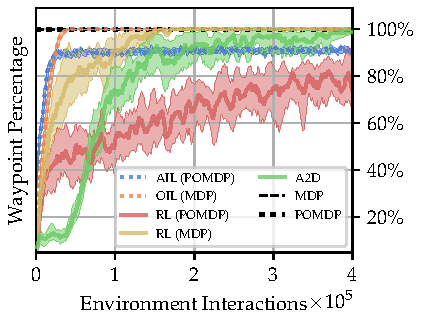
\includegraphics[width=0.335\textwidth]{figures/carla/scenario_1_time_steps_wpp_results.pdf}
    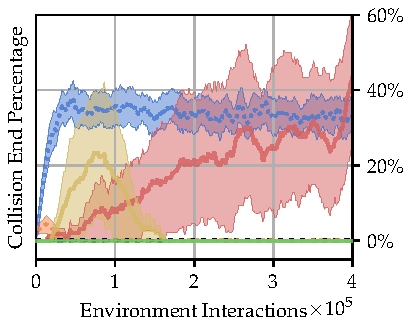
\includegraphics[width=0.33\textwidth]{figures/carla/scenario_1_time_steps_collision_results.pdf}
    \caption{Performance metrics for the AV scenario, introduced in Section \ref{sec:results}.  We show median and quartiles across ten random seeds.  Left: average cumulative reward.  Center: average percentage of waypoints collected, measuring progress along route.  Right: percentage of trajectories ending in a child collision.  Optimal MDP and POMDP solutions are shown by dashed and dotted lines respectively.  In methods marked as MDP the agent uses an omniscient compact state, including the child's state.  AIL (\emph{AIL (MDP)}) and RL (\emph{RL (MDP)}) learn a performant (high reward and waypoint percentage, low collision percentage) policy quickly and reliably.  In methods marked as POMDP the agent uses the high-dimensional monocular camera view.  Therefore, \emph{AIL} leads to a high collision, and the perception task makes RL in the POMDP (\emph{RL (POMDP)}) slow and variable (low reward and waypoint percentage, high collision percentage).  \emph{A2D} solves the scenario (high reward and waypoint percentage, low collision percentage) in a budget commensurate with the best-case convergence of \emph{RL (MDP)}.}
    \label{supp:fig:grid:a2dplot:results}
\end{figure*}



We implement this scenario in the CARLA simulator~\citep{Dosovitskiy17}, which is visualized in Figure \ref{supp:fig:carla:a2dplot:inputs}.  A child is present in 50\% of trials, and, if present, emerges with variable velocity.  The action space consists of the steering angle and amount of throttle/brake.  As an approximation to the optimal policy under privileged information, we used a hand-coded expert that completes the scenario driving at the speed limit if the child is absent, and slows down when approaching the truck if the child is present.  The differentiable expert is a small neural network, operating on a six-dimensional state vector that fully describes the simulator state.  The agent is a convolutional neural network that operates on grayscale images from the front-view camera. 

Results comparing A2D to four baselines are shown in Figure \ref{supp:fig:grid:a2dplot:results}.  \emph{RL (MDP)} uses RL to learn a policy conditioned on the omniscient compact state, only available in simulation, and hence does not yield a usable agent policy.  This represents the absolute best-case convergence for an RL method, achieving good, although not optimal, performance quickly and reliably.  \emph{RL} learns an agent conditioned on the camera image, yielding poor, high-variance results within the experimental budget. \emph{AIL} uses asymmetric DAgger to imitate the hand-coded expert using the camera image, learning quickly, but converging to a sub-optimal solution.  We also include \emph{OIL (MDP)}, which learns a policy conditioned on the omniscient state by imitating a hand-coded expert, and converges quickly to the near-optimal solution (\emph{MDP}). As expected, \emph{A2D} learns more slowly than AIL, since RL is used to update to the expert, but achieves higher reward than \emph{AIL} and avoids collisions.  This scenario, as well as any future asymmetric baselines, are distributed in the repository.  
